\documentclass[a4paper,12pt]{report}

\usepackage[utf8]{inputenc}
\usepackage[T1]{fontenc}
\usepackage{hyperref}
\usepackage{graphicx}
\usepackage{tabu}
\usepackage{longtable}
\usepackage{fullpage}
\usepackage{float}
\restylefloat{table}
\usepackage{listings}
\lstset{language=C,breaklines=true,breakautoindent=true}

\begin{document}

\title{\textbf{cAER}\\A framework for event-based processing\\on embedded and desktop systems}

\author{iniLabs Ltd.}

\date{\today}

\maketitle

\tableofcontents{}

\chapter{Introduction} \label{chap:introduction}

Embedded systems are prime candidates to fill this role of power-efficient computation units, but they also pose significant challenges in terms of software design, owing to their often very limited computing resources.

The current jAER project is written entirely in the Java programming language, which already poses a significant problem: many embedded systems do not posses a working Java Virtual Machine (JVM) implementation, and even on those that do, the overhead imposed by it may already be prohibitive to the kind of applications people are interested in. Further, jAER is reliant on a graphical user interface (GUI) for interactive control and output visualization, a feature that is rarely present on target systems such as autonomous robots, and that again requires significant computational resources and increases power consumption.

A new software needed to be written, that would take full advantage of the event-driven computation model, as well as being usable on a wide range of embedded systems, taking their limited available resources into account.
This work explores just such a software component, its architecture and its implementation.

The main target platforms were determined to be consumer-grade embedded systems, such as the Raspberry Pi, the PandaBoard, the Parallella or the Odroid embedded computers.

Based on the use cases above, the project goals and the mentioned issues (in chapter \ref{chap:introduction}) with the jAER framework, a number of requirements quickly emerged:
\begin{itemize}
\item able to run on a wide range of low-power, embedded systems
\item small memory footprint, conscious usage of CPU cores, no assumption that multiple of them will be present
\item able to run on the Linux operating system
\item able to communicate with external USB devices
\item focus on processing events generated by connected sensors
\item no focus on visualization, no dependency on any graphical user interface
\item network-enabled to communicate easily with other systems and frameworks (like jAER) or forward data to other processing nodes
\item able to run without supervision for long amounts of time
\item configurable without the need for graphical user interfaces, possibly configurable remotely
\item reusable code: framework structure and modularity
\end{itemize}

\chapter{Installation} \label{chap:installation}

\section{Manual Installation} \label{sec:manual_installation}

Given the stated goal of portability, the number of dependencies on external software had to be kept to a minimum, to avoid ones that might not build on a certain platform or require special hardware to run.
\clearpage
The following software is required to successfully compile cAER:
\begin{itemize}
\item A C compiler supporting the C99 language standard, as well as some GCC extensions (function/type attributes, inline assembler, synchronization intrinsics, thread-local storage), is needed to compile the code. GCC is currently the only compiler that meets all these requirements, starting with version 4.7.
\item A POSIX environment (Portable Operating System Interface), to supply threading, networking and file-system access functionality.
\item cmake 2.8+ for easy build management and cross-platform compilation support.
\item Mini-XML 2.7+ for XML file parsing, used for the XML configuration file import and export features.
\item DVS128 module: libusb 1.0.16+ (recommended 1.0.18+) to access USB devices from the application.
\end{itemize}

The installation procedure, once all dependencies are satisfied, is composed of four simple steps:
\begin{enumerate}
\item Get program sources
\item cmake .
\item Edit the main.c source-code file, to adjust the \emph{main()} function and define a custom Mainloop (further information can be found in sections \ref{subsec:main_definition} and \ref{subsec:mainloop_definition})
\item make
\end{enumerate}

At this point, the \emph{caer} executable, as well as its helper utilities, are ready for deployment and execution.

\section{Automatic Installation} \label{sec:automatic_installation}

\chapter{Architecture} \label{chap:architecture}

A work pattern of getting events from an input, the \emph{source}, then processing and filtering them, and finally moving them to an output, the \emph{drain}, and repeating those steps again and again (usually in a loop), is common to most event-based processing software, and also forms the basis for the architecture described here.

The choice of an appropriate programming language is central to any software project.
As discussed in chapter \ref{chap:introduction}, the Java programming language was found to be ill suited for the task at hand. In fact, any kind of interpreted or virtual machine based language would add similar overhead.
In the end, the C programming language was selected, for a number of reasons:
\begin{enumerate}
\item it's a minimal, low-overhead, low-level language.
\item wide support for it is available on all kinds of hardware; indeed many embedded systems or micro-controllers only have a C compiler and environment available.
\item it is well supported by all manners of different tools, from integrated development environments (IDEs) to static code analyzers.
\item it enjoys an enormous ecosystem of libraries, providing access to a large range of software and hardware functionality, many of clear interest for computational workloads (OpenCL, CUDA) or computer vision ones (OpenCV).
\end{enumerate}

\section{Framework} \label{sec:framework}

The stated goal of this work is to develop a new event-driven data processing framework suitable for low-power applications and high-speed sensors.
Such a framework should provide common functionality such as configuration management and logging, as well as handling all the data processing setup, such as starting up threads, processes, inputs and outputs.
It should offer the user a simple, well-defined way to put together the parts of the framework he needs for his application, and be easy to deploy across various systems.
It should further be easily possible to extend the functionality of the framework with self-written, application-specific code.

To this end it was decided to implement cAER as a collection of basic framework functionality and modules, which could easily be plugged and extended by the user.

A broad overview of the resulting architecture is shown in Figure \ref{fig:caer_architecture}. The various components will be explained in detail in the following sections, first from a high-level architectural point of view, and then from a more implementation-minded point of view in chapter \ref{chap:implementation}.

\begin{figure}[H]
\begin{center}
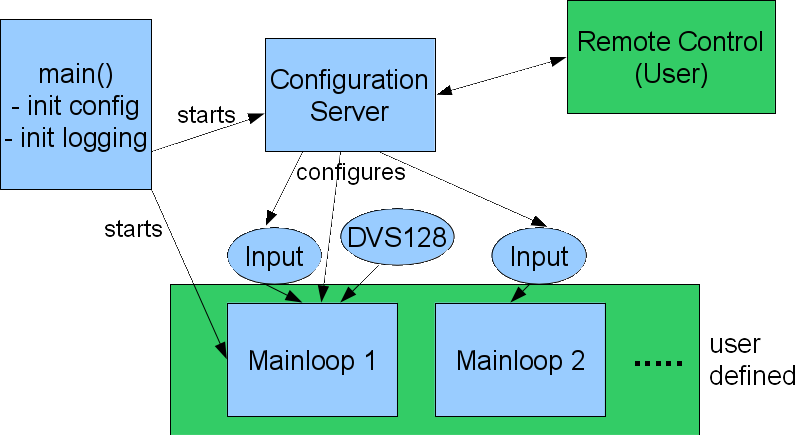
\includegraphics[width=\textwidth]{caer_architecture}
\caption{cAER architecture overview}
\label{fig:caer_architecture}
\end{center}
\end{figure}

The main program thread is responsible for setting up configuration and logging, and then start the rest of the framework. 
As such, each data processing loop runs inside its own thread, as well as each input.
A further thread is started for the run-time configuration system, to allow users to modify system settings at any time, while the other parts of the program are running.

The total number of running system threads is 2 (main thread + config thread).

\section{Events} \label{sec:events}

What an event represents, how to access it, the format of the data it contains, its storage requirements and memory layout, are all fundamental questions for any event-based processing software.

Events need to have several characteristics to meet the requirements determined before in section \ref{sec:requirements}:
\begin{itemize}
\item low memory consumption
\item fast data access
\item extensibility to future devices
\item low iteration overhead
\item low deletion overhead
\end{itemize}

When defining the new event format, a careful balance had to be maintained between memory consumption and amount of information that could be stored regarding future extensions. While it might be tempting to just use two 4-byte integers to encode the X and Y dimensions of an event coming from a camera pixel, to support devices with up to 4 GigaPixels per axis in theory, such sensors don't exist and won't exist for years to come, and this is even more true for the sensors developed at the Institute of Neuroinformatics, which have a reduced resolution due to increased pixel size and other factors. It then makes more sense to put both the X and Y values in one 4-byte integer, allocating each a fixed amount of bits, to conserve memory and especially storage bandwidth and capacity when transmitting events over the network or storing them to disk. With this method, it's possible to really minimize memory usage for each type of event individually.

Fast data access is still guaranteed, since, at most, accessing data stored with the above method would require an integer shift and AND operation, while storing data an integer shift and OR operation. Sometimes just an AND or OR operation, when the shift amount is zero. Such bit-wise operations are extremely fast on modern CPU architectures, usually taking just 1 CPU cycle. Intel for example reports latency values of 1 cycle for AND/OR instructions and 1 cycle for shifts (SHL/SHR instructions) for modern Haswell processors and for its Silvermont architecture (successor to Atom for low-power scenarios) \cite{intel_manual}.

To enhance iteration performance, and generally reduce the load that moving events from one processing stage to the other incurs; events are always grouped together into packets, and kept adjacent in memory. Going from event to event just requires a pointer increment, and moving a packet between processing stages just involves passing around a pointer to it.

A further benefit of grouping events into packets is that a packet header can be defined and used to store useful information about the events it contains, such as their type or source, in a non-redundant way, instead of putting that information with each event separately, further saving memory.

Finally, concerning the low deletion overhead, instead of implementing the removal of events by copying only the valid ones to a new packet, or shifting them around inside the current packet, a 1-bit boolean flag has been made a mandatory part of each event, indicating if the event is to be considered valid (flag is 1) or invalid (flag is 0). A side-benefit of this approach is that it is still possible for later processing stages to examine invalidated events, which might be interesting for example for statistics.

\url{https://inilabs.com/support/software/fileformat/#h.oqxw4mby5yg2}

The \emph{eventType} field stores the type of event that is contained in the packet.
Currently the following event types are defined:

The \emph{eventSource} field encodes a unique numeric ID that represents the input from which the event originates.
The ID is unique inside a data processing loop and can be used to retrieve information on the input in later processing stages that work on a particular packet.

getTimestamp/getTimestamp64

\section{XML Configuration} \label{sec:xml_configuration}

To this end, the Super Simple Hierarchical Storage (SSHS, \ref{subsec:sshs}) library was written and then employed. A configuration file from which to load the initial settings is also part of this system.

On the first execution of the \emph{caer} program, all configuration will be initialized to its default values.

Manipulating configuration values is possible either by using the \emph{caerctl} utility (see section \ref{subsec:caerctl}) at run-time, or by editing the XML configuration file that is written each time the program shuts down.
\clearpage
The following listing shows an excerpt from the configuration file in question:

\begin{lstlisting}
 1:<sshs version="1.0">
 2:  <node name="" path="/">
 3:    <node name="1" path="/1/">
 4:      <node name="2-FileOutput" path="/1/2-FileOutput/">
 5:        <attr key="directory" type="string">/home/caer</attr>
 6:        <attr key="prefix" type="string">caer_out</attr>
 7:        <attr key="validEventsOnly" type="bool">true</attr>
 8:      </node>
 9:      ...
10:    </node>
11:    ...
12:  </node>
13:</sshs>
\end{lstlisting}

The first line specifies that this file conforms to the SSHS format specification (from section \ref{subsec:sshs}), version 1.0.
After that, the tree-like hierarchical structure is clearly visible, with the root node (line 2) holding all Mainloops (line 3), which in turn hold all the modules (line 4).
The \emph{<attr>} tags contain the configuration values themselves, the \emph{key} attribute identifies and names the value, the \emph{type} attribute specifies its SSHS type, and the tag's value itself represents the effective configuration value.

In the above example, the \emph{validEventsOnly} configuration value is of boolean type, and can assume values of \emph{true} or \emph{false}.

To allow for consistent configuration updates inside the modules, changes to the configuration are only applied once per Mainloop cycle, by the module state machine, right before the actual data processing code is executed (see \emph{moduleConfig} in section \ref{sec:modules}).
Since changes to the configuration can happen at any time, due to the configuration server thread (see section \ref{subsec:remote_configuration}), a mechanism had to be developed to notify the running modules that a configuration refresh was desired on their next execution. A single, atomic variable in each module is used for the purpose of asynchronously signaling configuration changes, allowing the module to quickly determine on each run if it needs to update its configuration and react to eventual changes. This provides an efficient inter-thread communication solution, instead of relying on expensive locks to synchronize some additional state variable.
SSHS listeners are added to each module's configuration nodes, to set the above atomic variable appropriately when changes occur.

\section{Mainloop} \label{sec:mainloop}

As mentioned at the start of chapter \ref{chap:architecture}, the core of any kind of data processing architecture is represented by the following three steps:
\begin{itemize}
\item get data from (one or more) inputs (\emph{sources})
\item process / filter data
\item send data to (one or more) outputs (\emph{drains})
\end{itemize}
Such processing usually happens in a loop, getting new data as soon as being finished with the old one or at fixed intervals in time.

In event-driven data processing, and especially in low-power scenarios, the expectation is that those three steps only happen when the input actually has generated meaningful data that can be processed, not before, and possibly also not after, to still guarantee acceptable reaction times to new events.
The continuous repetition of the tree above steps still happens, but the start condition slightly changes to hinge on the availability of new events to process.

A simple and efficient implementation is still represented by a loop, which shall run the processing functions only when there is more data, or else wait for a small time constant, before checking the availability of data again.

In cAER this process is simply called the Mainloop, short for Main-Data-Processing-Loop.
Mainloops are defined by the user and connect inputs to processing modules and finally to outputs.
They represent the actual operations the user wants to repeatedly see happen on the data.
\clearpage
The thread-function that runs a Mainloop looks like this (in pseudo-code):

\begin{lstlisting}
while (run_system) {
    if (data_is_available) {
        execute_mainloop_definition();
    }
    else {
        sleep(1 ms);
    }
}
\end{lstlisting}

\subsection{Asynchronous inputs} \label{sec:asynchronous_inputs}

To be able to run the Mainloop only when data is available, something else has to be running and making that data available. The input modules have a secondary part, which is executing inside a separate thread, and is responsible for getting the bare data from connected devices, network streams or files, and signaling its availability to the Mainloop (the data\_is\_available variable in the pseudo-code above).

The input threads themselves employ techniques, such as blocking I/O, or asynchronous USB transfers, that also limit activity to only when data is available at the device or network level, to avoid unnecessary overhead. At this point, minimal processing is performed to interpret the data and format it according to the event packet definitions from section \ref{sec:events}, and then the data is made available to the Mainloop.
The actual exchange of data between the two threads happens by means of a special lock-free variant of a ring-buffer, a high-performance, array-based data structure.

Memory allocated by the input threads is later automatically reclaimed after the current cycle of the Mainloop has completed, completely removing this particular concern from the user.

\section{Modules and Connectivity} \label{sec:modules_and_connectivity}

\chapter{Usage} \label{chap:usage}

\section{caer-config.xml}

\section{caer-bin}

It also tries to interpret any given command-line parameters and uses their values to set and override previous configuration settings.
The command-line override takes the following format and can be repeated multiple times to override multiple options:
\\\emph{-o <node string> <key string> <key type string> <value string>}

The configuration file-name parameter can be either an absolute path to a file or a single file-name, which is treated as residing inside the current working directory of the program.
It is possible to disable the loading and saving of the settings to the configuration file by passing NULL as a value instead of a file-name.

\section{Modules}

\subsection{DVS128} \label{subsec:dvs128}

\begin{lstlisting}
void caerInputDVS128(uint16_t moduleID, caerPolarityEventPacket *polarity, caerSpecialEventPacket *special);
\end{lstlisting}

This input module allows a DVS128 camera to be connected and events to be captured from it.
As can be seen from its function signature above, it generates polarity event packets and special event packets, by putting their address into the given pointer. If no event packets of a certain type are available at the moment, NULL is assigned instead. This is done to not delay the current Mainloop cycle if certain types of produced events are much more scarce than others. To indicate that one is not interested at all in an event packet of a certain type, NULL can be passed to the function instead of a pointer.

As explained in section \ref{sec:asynchronous_inputs}, this module starts a separate thread, the Data Acquisition Thread, that reads the events from the hardware device and transforms them into suitable event packets, as defined in section \ref{sec:events}, and then passes them on for further processing to the Mainloop.
This module uses the libusb library for accessing the DVS128 camera, which is connected to its host via a USB 2.0 interface. For higher performance, asynchronous USB transfers are employed.

Multiple cameras can be connected and accessed by calling this module multiple times: each instance will then be connected to one camera. The order in which cameras are accessed is based on the host USB bus and device numbers, lower numbers being accessed first by module instances appearing before in a Mainloop. Across different Mainloops, the order is undefined.

If no camera is currently connected to the host system, the module will attempt to connect to one on each Mainloop cycle. Conversely, if a connected camera is physically disconnected, the module will detect this and shut itself down.

The DVS128's configuration node offers the following settings for customization:
\begin{description}
\item[bufferNumber] the number of the USB buffers currently being used for asynchronous data transfers with the device.
\subitem Type: int, Default value: 8
\item[bufferSize] the size in bytes of the USB buffers currently being used for asynchronous data transfers with the device.
\subitem Type: int, Default value: 4'096 bytes
\item[dataExchangeBufferSize] the number of elements the ring-buffer used to transfer event packets from the Data Acquisition Thread to the Mainloop can hold before it gets full and starts rejecting newly produced packets.
\subitem Type: int, Default value: 64
\item[polarityPacketMaxInterval] the maximum time interval in $\mu$s between the first and the last event in a polarity event packet, after which it is transferred to the Mainloop.
\subitem Type: int, Default value: 5'000 $\mu$s
\item[polarityPacketMaxSize]  the maximum number of events in a polarity event packet, after which it is transferred to the Mainloop.
\subitem Type: int, Default value: 4'096
\item[shutdown] enables or disables this module.
\subitem Type: bool, Default value: false
\item[specialPacketMaxInterval] the maximum time interval in $\mu$s between the first and the last event in a special event packet, after which it is transferred to the Mainloop.
\subitem Type: int, Default value: 1'000 $\mu$s
\item[specialPacketMaxSize] the maximum number of events in a special event packet, after which it is transferred to the Mainloop.
\subitem Type: int, Default value: 128
\end{description}

A sub-node called \emph{/bias/} is also provided to set the DVS128's bias currents.
The following biases are specified as integer settings: \emph{cas, diff, diffOff, diffOn, foll, injGnd, pr, puX, puY, refr, req, reqPd}. Their default values are based on the official fast bias settings for the DVS128 from the jAER project \cite{jaer_project} repository (DVS128Fast.xml in jAER/trunk/biasgenSettings/DVS128/).

The \emph{/sourceInfo/} sub-node defines the following values that can be queried by other modules:
\begin{description}
\item[sizeX] the X axis resolution for this camera in pixels.
\subitem Type: short, Default value: 128 pixels
\item[sizeY] the Y axis resolution for this camera in pixels.
\subitem Type: short, Default value: 128 pixels
\end{description}
\subsection{eDVS}
\subsection{DAVIS}
\subsection{Dynap-SE}
\subsection{Background Activity Filter} \label{subsec:backgroundactivityfilter}

\begin{lstlisting}
void caerBackgroundActivityFilter(uint16_t moduleID, caerPolarityEventPacket polarity);
\end{lstlisting}

The Background Activity Filter takes polarity event packets and invalidates any polarity event that is not supported by other polarity events in its neighborhood within a certain time window.
It implements this by looking up the latest timestamp before the current one in a map and comparing the difference against a fixed threshold value set by the user.
This considerably reduces the background noise generated by the camera and helps in clearing up its output.
\clearpage
The following settings are recognized:
\begin{description}
\item[deltaT] maximum time-difference in $\mu$s between the current event and the last supported activity by one of its neighbors, after which events are declared invalid.
\subitem Type: int, Default value: 30'000 $\mu$s
\item[shutdown] enables or disables this module.
\subitem Type: bool, Default value: false
\item[subSampleBy] sub-sample by shifting the x and y values by this many positions. This results in a logical halving of the map size on both axes for each shift.
\subitem Type: byte, Default value: 0
\end{description}
\subsection{Visualizer}

Windows: print to Windows Command Console is very slow, disable the Statistics module, use a high log-level.

\subsection{Camera Calibration}
\subsection{Frame Enhancer}
\subsection{Frame Statistics}
\subsection{Statistics}
\subsection{Pose Estimation}
\subsection{Median Tracker}
\subsection{Rotate Filter}

\subsection{File} \label{subsec:file}

\begin{lstlisting}
void caerOutputFile(uint16_t moduleID, size_t outputTypesNumber, ...);
\end{lstlisting}

The file output module writes event packets directly to a file.
The following scheme is utilized to generate the file-name:
\\\emph{<directory>/<prefix>-YEAR-MONTH-DAY\_HOUR:MINUTE:SECOND.aer2}
\\The user controls the directory and prefix parts, and a suffix containing the current time is appended, so as to always supply start-of-recording temporal information automatically.
The AER2 file extension signals that a new file format is being used, based on the event packets as defined in section \ref{sec:events}.

It can take an arbitrary number of event packets and types, and will output them in the order they are given. The total number of output packets has to be specified for this to work correctly.

The user may specify if the full event packet (valid and invalid events) shall be written, or just the valid events. Writing only the valid events incurs a small performance penalty, since they have to be separated from the invalid ones.
\clearpage
The following settings are recognized:
\begin{description}
\item[directory] the directory where data files will be saved to.
\subitem Type: string, Default value: <user home directory>
\item[prefix] the file-name prefix part.
\subitem Type: string, Default value: caer\_out
\item[shutdown] enables or disables this module.
\subitem Type: bool, Default value: false
\item[validEventsOnly] only output valid events, discarding the invalid ones.
\subitem Type: bool, Default value: false
\end{description}

\subsection{Unix socket client} \label{subsec:unix_socket_client}

\begin{lstlisting}
void caerOutputUnixS(uint16_t moduleID, size_t outputTypesNumber, ...);
\end{lstlisting}

The Unix socket client output module writes event packets directly to a local Unix socket and is the preferred way to send data to another process on the same machine. Order and reliability of the communication are guaranteed.
The specified local Unix socket must already have been created by another process that wants to receive data from cAER and be in listening mode (see the \emph{unixststat} utility source-code for an example).

It can take an arbitrary number of event packets and types, and will output them in the order they are given. The total number of output packets has to be specified for this to work correctly.

The user may specify if the full event packet (valid and invalid events) shall be sent, or just the valid events. Sending only the valid events incurs a small performance penalty, since they have to be separated from the invalid ones.

The following settings are recognized:
\begin{description}
\item[shutdown] enables or disables this module.
\subitem Type: bool, Default value: false
\item[socketPath] the path to the local Unix socket to connect with.
\subitem Type: string, Default value: /tmp/caer.sock
\item[validEventsOnly] only output valid events, discarding the invalid ones.
\subitem Type: bool, Default value: false
\end{description}
\clearpage
\subsection{UDP network client} \label{subsec:udp_network_client}

\begin{lstlisting}
void caerOutputNetUDP(uint16_t moduleID, size_t outputTypesNumber, ...);
\end{lstlisting}

The UDP network client output module sends event packets directly over an UDP connection to a remote host.
The UDP protocol guarantees neither ordered transmission nor transmission reliability, and should thus only be used on the local network, where the user has more control over what's happening, or in situations where data loss is potentially acceptable, and where the higher efficiency of UDP, due to decreased protocol overhead, outweighs the risks. In all other cases, the use of TCP is recommended.
Given the connection-less nature of the UDP protocol, no checking is performed to verify if, on the specified remote host, there really is some process ready to listen to the data being sent. Data packets are simply sent out and then "forgotten" from the point of view of the cAER framework.

It can take an arbitrary number of event packets and types, and will output them in the order they are given. The total number of output packets has to be specified for this to work correctly.

The user may specify if the full event packet (valid and invalid events) shall be sent, or just the valid events. Sending only the valid events incurs a small performance penalty, since they have to be separated from the invalid ones.

The following settings are recognized:
\begin{description}
\item[ipAddress] the IP address of the remote host to send packets to.
\subitem Type: string, Default value: 127.0.0.1
\item[portNumber] the destination port on the remote host to send packets to.
\subitem Type: short, Default value: 8888
\item[shutdown] enables or disables this module.
\subitem Type: bool, Default value: false
\item[validEventsOnly] only output valid events, discarding the invalid ones.
\subitem Type: bool, Default value: false
\end{description}

\subsection{TCP network client} \label{subsec:tcp_network_client}

\begin{lstlisting}
void caerOutputNetTCP(uint16_t moduleID, size_t outputTypesNumber, ...);
\end{lstlisting}

The TCP network client output module sends event packets directly over a TCP connection to a remote host.
TCP is a reliable, in-order, connection-oriented protocol. As such, for the connection to succeed, a TCP server must be ready and waiting for connections on the specified remote host.

It can take an arbitrary number of event packets and types, and will output them in the order they are given. The total number of output packets has to be specified for this to work correctly.

The user may specify if the full event packet (valid and invalid events) shall be sent, or just the valid events. Sending only the valid events incurs a small performance penalty, since they have to be separated from the invalid ones.

The following settings are recognized:
\begin{description}
\item[ipAddress] the IP address of the remote host to connect to.
\subitem Type: string, Default value: 127.0.0.1
\item[portNumber] the destination port on the remote host to connect to.
\subitem Type: short, Default value: 8888
\item[shutdown] enables or disables this module.
\subitem Type: bool, Default value: false
\item[validEventsOnly] only output valid events, discarding the invalid ones.
\subitem Type: bool, Default value: false
\end{description}

\subsection{TCP network server} \label{subsec:tcp_network_server}

\begin{lstlisting}
void caerOutputNetTCPServer(uint16_t moduleID, size_t outputTypesNumber, ...);
\end{lstlisting}

The TCP network server output module starts a TCP server on the local host and waits for connections from other systems. Once a remote system has completed the connection procedure, the output module sends event packets directly over the established TCP connection to the remote system.
The simple action of connecting to this server by a client and successfully completing the connection procedure, taking into account the maximum number of allowed clients, puts it into the list of clients that data is sent to, starting the data transfer right away.
Closing the connection on the client's part takes them off this list, putting a stop to the data transfer.
A change to the maximum number of connected clients also has repercussions on already connected ones: if the new value is smaller than the number of currently connected clients, some of them will be disconnected to adhere to the new quota.

It can take an arbitrary number of event packets and types, and will output them in the order they are given. The total number of output packets has to be specified for this to work correctly.

The user may specify if the full event packet (valid and invalid events) shall be sent, or just the valid events. Sending only the valid events incurs a small performance penalty, since they have to be separated from the invalid ones.
\clearpage
The following settings are recognized:
\begin{description}
\item[backlogSize] maximum number of pending connections kept in the connection queue.
\subitem Type: short, Default value: 5
\item[concurrentConnections] maximum number of allowed simultaneously connected clients.
\subitem Type: short, Default value: 5
\item[ipAddress] the local IP address on which to have the server listen for incoming connections.
\subitem Type: string, Default value: 127.0.0.1
\item[portNumber] the local port on which to have the server listen for incoming connections.
\subitem Type: short, Default value: 7777
\item[shutdown] enables or disables this module.
\subitem Type: bool, Default value: false
\item[validEventsOnly] only output valid events, discarding the invalid ones.
\subitem Type: bool, Default value: false
\end{description}

\section{Command-Line Utilities} \label{sec:cli_utilities}

Several command-line utilities are distributed together with the \emph{caer} program:
\begin{description}
\item[caerctl] is used to query and set configuration values while the \emph{caer} program is running.
\item[unixststat] provides a quick way to test the local Unix socket client output and print information on incoming traffic from that output.
\item[udpststat] provides the same for the UDP network client output.
\item[tcpststat] again provides similar functionality for the TCP network server output.
\end{description}

\subsection{caerctl} \label{subsec:caerctl}

The \emph{caerctl} utility takes exactly two arguments: an IP address and a port, to which a connection attempt will be made. At this address, a \emph{caer} instance with a reachable configuration server should be running.
If no arguments are specified, the default IP:port values of \emph{127.0.0.1:4040} are used.
Once \emph{caerctl} has connected successfully with the remote configuration server, the following commands are available for the user to type in and submit:
\begin{description}
\item[node\_exists:] checks whether a node exists or not.
\subitem Usage: node\_exists <node string>
\item[attr\_exists:] checks whether a node's attribute exists or not.
\subitem Usage: attr\_exists <node string> <key string> <key type string>
\item[get:] queries the current value of the specified attribute.
\subitem Usage: get <node string> <key string> <key type string>
\item[put:] sets the value of the specified attribute to the supplied one.
\subitem Usage: put <node string> <key string> <key type string> <value string>
\item[quit or exit:] disconnects from the configuration server and closes the program.
\subitem Usage: quit / exit
\end{description}

To simplify interaction with the user and not require him to remember all the configuration paths, automatic command-completion has been implemented, by using the GET\_CHILDREN, GET\_ATTRIBUTES and GET\_TYPES actions from section \ref{subsec:remote_configuration}.
By pressing the TAB key, the user will be presented with a list of possible completions to select from. Further completions are cycled by pressing TAB again, until returning to the original starting point. Unambiguous completions are selected automatically; in case of multiple choices, the SPACE key confirms the current choice.
Command history is also provided, one can navigate to previous commands and back with the UP and DOWN arrow keys, and the commands entered during previous \emph{caerctl} sessions are saved to a file named \emph{.caerctl\_history} in the user's home directory, and made available again on the next session.

The implementation of such functionality requires support from an external library, three of them were evaluated: GNU Readline was the first choice and discarded because of the forced GPLv2 license, which might have prevented certain commercial and industrial users from seriously considering cAER. The mediocre documentation did not help. Editline was discarded because of problems in getting the contents of the currently being typed line of text, at least while in Readline-compatibility mode. Again, the scarce documentation did not help clear matters up.
In the end the choice fell on Linenoise, a very small library that implements the most basic functionality needed, while also allowing easier integration into a project by just requiring direct inclusion of two small source-code files and avoiding any licensing restrictions by employing the BSD license.

\subsection{unixststat} \label{subsec:unixststat}

The \emph{unixststat} utility takes exactly one argument: an absolute file-system path, where a local Unix socket will be created and configured in listening mode.
If no arguments are specified, the default socket path value of \emph{/tmp/caer.sock} is used.
A continuous stream of information on the incoming data packets will then be printed on the console.

\subsection{udpststat} \label{subsec:udpststat}

The \emph{udpststat} utility takes exactly two arguments: a local IP address and a port, on which to start listening for incoming UDP packets.
If no arguments are specified, the default IP:port values of \emph{127.0.0.1:8888} are used.
A continuous stream of information on the incoming data packets will then be printed to the console.

\subsection{tcpststat} \label{subsec:tcpststat}

The \emph{tcpststat} utility takes exactly two arguments: an IP address and a port, to which a connection attempt will be made. At this address, a \emph{caer} instance with a reachable TCP network server output module (described in section \ref{subsec:tcp_network_server}) should be running.
If no arguments are specified, the default IP:port values of \emph{127.0.0.1:7777} are used.
A continuous stream of information on the incoming data packets will then be printed to the console.

\section{GUI Utilities} \label{sec:gui_utilities}

\subsection{caerctl-gui-javafx}

\chapter{Development} \label{chap:development}

\section{Structure} \label{sec:structure}

The implementation is divided into multiple files and directories, to allow for a clean separation of concerns.

The main.c source-code file connects all the parts into a working program, as detailed in section \ref{sec:application_definition}.

The base/ directory contains all the framework functionality, explained in section \ref{sec:framework} and onwards.

The events/ directory houses all the definitions of the events and their packets, according to the format discussed in section \ref{sec:events}.
All event definitions, as well as the common packet header definition, are implemented as stand-alone, reusable header files, to promote and simplify integration with other projects, which will easily be able to interpret data coming from cAER by including these files.

ext/ contains external libraries that are used throughout the program, as well as internal ones such as SSHS that were developed specifically for this project (see section \ref{subsec:sshs}).

The modules/ folder contains all the input (section \ref{sec:input_modules}), processing (section \ref{sec:processing_modules}) and output (section \ref{sec:output_modules}) modules, that a user may employ for his application.

Finally, the utilities/ folder contains small helper programs, detailed in section \ref{sec:utilities}.













It gets the relevant settings from the configuration sub-system's \emph{/logger/} node; those are:
\begin{description}
\item[logFile] the file where log messages are stored.
\subitem Type: string, Default value: <current working directory>/caer.log
\item[logLevel] the cut-off level for log messages. Messages of lesser importance are ignored.
\subitem Type: byte, Default value: 5 (corresponds to LOG\_NOTICE as shown in section \ref{sec:logging})
\end{description}

The configuration server stores its own settings in the \emph{/server/} node:
\begin{description}
\item[backlogSize] maximum number of pending connections kept in the connection queue.
\subitem Type: short, Default value: 5
\item[concurrentConnections] maximum number of allowed simultaneously connected clients.
\subitem Type: short, Default value: 5
\item[ipAddress] IP address on which to listen for connections.
\subitem Type: string, Default value: 127.0.0.1
\item[portNumber] port number on which to listen for connections.
\subitem Type: short, Default value: 4040
\end{description}

\section{Input modules} \label{sec:input_modules}

Input modules provide events to a Mainloop.

Each input module defines a configuration sub-node called \emph{/sourceInfo/}, which contains constants and other read-only information about the module and the events it produces. This can then be accessed by other modules to find out values such as the size in pixels of a camera or the number of audio channels available.

One limitation exists: the same input module accessing the same underlying event producer (hardware device, network stream, file, ...) cannot exist more than once across all Mainloops. Sharing the same input over multiple Mainloops would require expensive copying and distribution of data, which is best avoided in resource constrained environments.
Hardware device access modules usually try to get exclusive access to their device, rendering this kind of error impossible: a second instance of the same module accessing the same device would simply not be able to open it.
\clearpage


\section{Processing modules} \label{sec:processing_modules}

Processing modules modify the data contained in event packets, or can even create new ones with new types of data, based on their input.

Any processing module should be prepared to have a NULL value instead of an event packet being handed to it, this can happen for example when no event packets of that type were available from the preceding input modules at that moment in time.

\section{Output modules} \label{sec:output_modules}

Once elaborated, the events need to be either saved or redirected somewhere, be it for further processing or to control external hardware, such as a robotic arm: output modules are the ones responsible for this operation.

Any output module should be prepared to have a NULL value instead of an event packet being handed to it, this can happen for example when no event packets of that type were available from the preceding input modules at that moment in time.
Checking that there are valid events on which to work is also usually a good idea, since an event packet might have been completely invalidated by preceding processing modules, and factually be "empty" of any useful data, at the time it reaches an output module.

Event packets are sent directly 1:1 over the network or stored to file. This reduces the additional processing to be done at output time, in the common case, to nothing.

\section{SSHS} \label{subsec:sshs}

SSHS is a stand-alone library that provides in-memory, hierarchical, structured information storage capabilities.
It is inspired by the Java Preferences system, but with a better control of where its content is stored and when it's written out to disk, which happens exclusively on the explicit request of the user.
The content of the hierarchical storage can be exported to XML for easy sharing, improved human readability and editing, and such XML files can also be imported back to initialize or update the storage's content.

It implements a tree-like structure, with nodes that contain links to other nodes (their children), as well as attributes.
To retrieve a specific node, absolute paths from the root node (\emph{/this/is/an/absolute/path/}) or relative paths from an ancestor node (\emph{a/relative/path/}) can be utilized. Functions to verify the existence of nodes are also present.

The attributes contain the actual data, which can be of eight types: boolean, byte (8-bit integer), short (16-bit integer), int (32-bit integer), long (64-bit integer), float, double and string.
Each attribute is uniquely identified by its type in combination with a string identifier.
Functions to get and set attribute values are provided:

list them
also C++ std::string variants

Getting an attribute is only possible if the attribute was declared beforehand, by either loading it from an XML file or by creating it using CREATE HERE.
This ensures that a valid value is present, and avoids having to specify a default value on each Get() call, as has to be done, for example, in the Java Preferences system.

Listeners can be added to nodes to react to changes to both the node's children and to its attributes.

FLAGS

\section{Remote configuration} \label{subsec:remote_configuration}

SSHS (see section \ref{subsec:sshs}) provides the actual mechanism to store, notify, and, together with the modules, apply configuration changes. Given the nature of cAER, which might run as a background process, an external interface was required for the user to actually tell the program what configuration changes should be done.

This interface was implemented as a TCP network server, listening on a user-configurable IP address and port combination, and allowing concurrently connected users to operate on the SSHS back-end and change the values of settings (attributes).
TCP was chosen for its reliability and ordering guarantees, as it would be unacceptable to loose configuration updates in transit over the network, or have them applied in an arbitrary order.
\clearpage
To communicate the details of a request, a custom protocol was implemented.
Control messages have the following format:
\begin{itemize}
\item 1 byte for the action
\item 1 byte for the type (representing SSHS types)
\item 8 bytes for length information:
\subitem 2 bytes extra field length
\subitem 2 bytes node length
\subitem 2 bytes key length
\subitem 2 bytes value length
\item then up to 4'086 bytes split between the extra field, the node, the key and the value strings. Each part, if present, must be NUL terminated, and the length shall also include the terminating NUL byte.
\end{itemize}
This results in a maximum message size of 4'096 bytes (4 KB).

The extra field is currently unused, and as such its length should always be zero. Its purpose is to allow future enhancements, such as authentication of requests.

The following requests can be made to the configuration server:

\begin{table}[H]
\begin{center}
\caption{Configuration server requests}
\label{tab:configuration_server_requests}
\begin{tabu} to \linewidth {|l|l|X|X|X|X|}
\hline
Action & Code & Type & Node & Key & Value \\ \hline
NODE\_EXISTS & 0 & 0 (unused) & absolute path & no & no \\ \hline
ATTR\_EXISTS & 1 & any & absolute path & key string & no \\ \hline
GET & 2 & any & absolute path & key string & no \\ \hline
PUT & 3 & any & absolute path & key string & value string \\ \hline
GET\_CHILDREN & 5 & 0 (unused) & absolute path & no & no \\ \hline
GET\_ATTRIBUTES & 6 & 0 (unused) & absolute path & no & no \\ \hline
GET\_TYPES & 7 & 0 (unused) & absolute path & key string & no \\ \hline
\end{tabu}
\end{center}
\end{table}
\clearpage
The response from the server follows a simplified version of the request protocol:
\begin{itemize}
\item 1 byte for the action
\item 1 byte for the type (representing SSHS types)
\item 2 bytes message length
\item then up to 4'092 bytes of response message. The message must again be NUL terminated, if present, and the NUL byte shall be included in the length calculation.
\end{itemize}
This results again in a maximum message size of 4'096 bytes (4 KB).

The server always responds either with an error (action code 4) or with a valid answer, with the same action code as the initial request.
The following table explains the response message format for the various actions that could have been submitted during the request phase:

\begin{table}[H]
\begin{center}
\caption{Configuration server responses}
\label{tab:configuration_server_responses}
\begin{tabu} to \linewidth {|l|l|X|X|}
\hline
Action & Code & Type & Message \\ \hline
ERROR & 4 & string & error string \\ \hline
NODE\_EXISTS & 0 & bool & true/false \\ \hline
ATTR\_EXISTS & 1 & bool & true/false \\ \hline
GET & 2 & same as request & result string \\ \hline
PUT & 3 & bool & true \\ \hline
GET\_CHILDREN & 5 & string & concatenation of string child names \\ \hline
GET\_ATTRIBUTES & 6 & string & concatenation of string attribute keys \\ \hline
GET\_TYPES & 7 & string & concatenation of string type names for a key \\ \hline
\end{tabu}
\end{center}
\end{table}

Thanks to this scheme, it is easily possible to implement an automatic discovery of the topology of the configuration back-end structure with the GET\_CHILDREN, GET\_ATTRIBUTES and GET\_TYPES actions, in addition to standard check, get and set functionality, thanks to the NODE\_EXISTS, ATTR\_EXISTS, GET and PUT actions.

\section{Logging} \label{sec:logging}

A logging system is a key component of any framework, since being able to output messages in a consistent way, with additional information such as the current system time, is quite important to inform the user of what's happening and assist in debugging failures.

Program code can call the \emph{caerLog()} logging function, giving it an importance level and a message. The message will only be logged if it happens to be more important than a user-set threshold, allowing efficient filtering of unimportant and undesired messages.
The following log levels are recognized:

\begin{table}[H]
\begin{center}
\caption{Log levels}
\label{tab:log_levels}
\begin{tabu} to \linewidth {|l|c|}
\hline
Log level & Code \\ \hline
LOG\_EMERGENCY & 0 \\ \hline
LOG\_ALERT & 1 \\ \hline
LOG\_CRITICAL & 2 \\ \hline
LOG\_ERROR & 3 \\ \hline
LOG\_WARNING & 4 \\ \hline
LOG\_NOTICE & 5 \\ \hline
LOG\_INFO & 6 \\ \hline
LOG\_DEBUG  & 7 \\ \hline
\end{tabu}
\end{center}
\end{table}

All messages are written out to a log file, to ensure their persistence, for later analysis.
For more immediate visual feedback, messages are also written out to the console, if cAER is not in daemon mode (see section \ref{subsec:daemon_mode}), which would render this impossible.

\section{Modules} \label{sec:modules}

Modules form the core of all data processing within cAER.
They implement ways for data to be made available (input modules), for it to be elaborated (processing modules) and for it to be sent somewhere else (output modules).

Each module is composed of a main function, which takes as parameters an unique module ID, as well as any needed input and output parameters, and this is the function called by users when defining the Mainloops.
This function is pretty simple in its content: it's responsible for retrieving the persistent module data and then calling the module state machine.

The module state machine takes care of initializing, running, configuring and shutting down a module, in such a way that each module can be disabled and reactivated while the Mainloop is still running, to easily test the effects that a module's presence or absence has on the data stream.
Each module can also allocate a region of memory to store permanent state that is to be accessible on each Mainloop cycle, such as maps, numbers, lists and so on.
Every module defines up to four functions that the state machine calls to do its work; the only required function is the \emph{moduleRun} function. The other three functions are optional, but most modules will want to implement them: the \emph{moduleInit} function takes care of initializing a module, ensuring all configuration values are present and have appropriate default values, initializing any memory and variables, etc.; its counterpart \emph{moduleExit} is responsible for cleaning up any resources at shutdown. The remaining function, \emph{moduleConfig}, contains the code that shall be executed when one of the module's configuration settings is changed by the user.
All module functions must be able to complete their work in one Mainloop cycle, they cannot for example shut down in multiple stages. This is also enforced by these functions being required to not return any value that might indicate their failure or success: they must always succeed. The sole exception is the \emph{moduleInit} function, which may return a boolean value of \emph{false}, if initialization was not possible (due to a missing device, not enough memory, wrong configuration settings, ...), in which case initialization will be reattempted on the next Mainloop cycle. This does not allow multi-stage initialization, as there is no persistent memory between successive \emph{moduleInit} calls that could be used to implement it.

The following pseudo-code illustrates the working of the module state machine, as is called on every Mainloop cycle:

\begin{lstlisting}
// 'moduleStatus' contains the current module status.
// 'running' specifies the wanted status: running or not.

if (moduleStatus == RUNNING && running == YES) {
    if (configuration was updated) {
        if (moduleFunctions->moduleConfig is defined) {
            moduleFunctions->moduleConfig(moduleData);
        }
    }

    moduleFunctions->moduleRun(moduleData, argsNumber, args);
}
else if (moduleStatus == STOPPED && running == YES) {
    if (moduleFunctions->moduleInit is defined) {
        if (!moduleFunctions->moduleInit(moduleData)) {
            return;
        }
    }

    moduleStatus = RUNNING;
}
else if (moduleStatus == RUNNING && running == NO) {
    moduleStatus = STOPPED;

    if (moduleFunctions->moduleExit is defined) {
        moduleFunctions->moduleExit(moduleData);
    }
}
\end{lstlisting}

\subsection{Modules API}

\section{Writing a new module}

\subsection{C++ support}

state memory in C++ must use pointers or explicit placement new/destructor calls, due to memory being
allocated with malloc/free.

\section{Porting old modules}

\section{Visualizer: Renderer and Event Handlers}

\end{document}
